\documentclass[11pt]{scrartcl}
\usepackage[T1]{fontenc}
\usepackage[utf8]{inputenc}

\title{Computer Systems Assignment 1}
\author{Daniel Coady (102084174) -- 12:30 Wednesday}
\date{25/08/2019}

\usepackage{graphicx}
\usepackage{fancyhdr}
\pagestyle{fancy}
\lhead{Daniel Coady (102084174)}
\rhead{COS10004 Computer Systems -- Assignment 1}

\begin{document}

\maketitle

\pagebreak

\section*{Stage 1}
\begin{figure}[h]
    \centering
    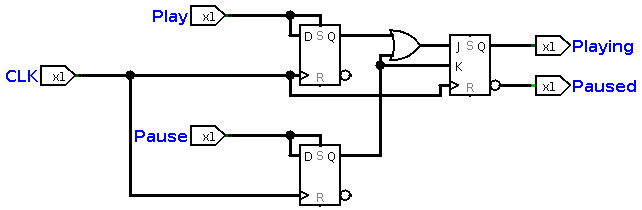
\includegraphics[scale=0.5]{images/stageone.png}
    \caption{Circuit used for stage one -- Play/pause functionality}
\end{figure}
For this stage I have assumed that we are to use a single pin/button to toggle on or off
the music player. Because of this I have used a single D flip-flop with the outputs Q and
Q' connected to the playing and paused outputs respectively.

\section*{Stage 2}
\begin{figure}[h]
    \centering
    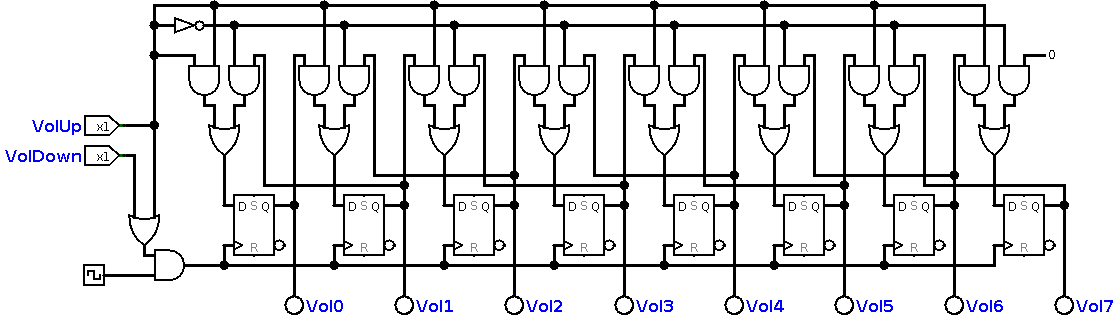
\includegraphics[scale=0.372]{images/stagetwo.png}
    \caption{Circuit used for stage two -- Volume control}
\end{figure}
This stage was a considerable amount more complicated than the last, and it has a circuit
to match. For this I assumed that the pins/buttons could continuously make the volume go
up or down. With this assumption in mind, I found it to be most appropriate to use a
bi-directional shift register to control volume values. This is for two reasons:

\begin{itemize}
    \item It allows for easy raising or lowering of the required bar graph display
    \item It inherently does not allow for overflowing or underflowing values
\end{itemize}

Of course, this isn't just a bi-directional shift register. I've made some modifications to
the inputs of circuit so that it may fit our application better. There are two inputs to
this ciruit: the volume up and volume down pins. Both of these pins are connected to an
or gate which feeds into an and gate that also has the clock as the input. This allows us
to control when we allow the clock pulse to feed into the circuit so that it can hold state
and not cause any unexpected behaviour.

\bigskip

This design is not without flaws however, since if you put both inputs on then it will simply
continue increasing the volume. I did attempt to fix this by replacing the or gate with a
xor gate, but this had it's own issue. When the xor gate was in use, occasionally when you go
from having both inputs on to just having the volume down input on it would go all the way to
zero from any state, which is not behaviour that we want. This may be solvable with a latch
to time the inputs to the clock, but I haven't been able to apply this yet. As such, I chose
the solution that gives the most consistent and useful output to the user.

\end{document}
